\chapter{Literature review}
This chapter aims to review the various types of mashups. It provides details that were researched by reading the academic papers and cites work that influenced the developing of our semantic mashup. In particular, general mashup architectures are studied, and the design process is thoroughly researched. Our focus is mainly on semantic mashups. Thereafter, a study of the problems and challenges encountered in designing such mashups are studied and analyzed.

\section{Research on web Mashups}
Mashups are distinguished based on their data and the services they provide. According to the programmable web \cite{23}, a huge number of mashups exist. Due to the abundance of data and services available, even end users are able to create simple mashups, based on predefined templates. A typical architecture of a mashup is usually divided in three layers \cite{4}:
\begin{enumerate}
\item \textbf{Content source:} These sources will have the data embedded in their web pages. Normally, some web sites provide APIs for their data systems which can be used for showing the data. Although some content providers may not have an implementable API yet, there are ways to get around this and employ techniques of screen scraping to gather data of interest. Content sources for our mashup are the web pages of interest from different web sites that contain the data on restaurants.
\item \textbf{Mashup UI:} This is the user interface for the semantic mashup application. This represents the presentation layer and user interfaces of mashups can be customized according to various needs. A proper design of the user interface can determine whether an interactive user experience can be provided. For instance, the user inserts a query with the UI and the query is processed and the results obtained are presented in an aesthetically pleasing way potentially based on user preferences. Client-side applications are normally used but server-side solutions exist as well.
\item \textbf{Platform:} This is often disputed as a third layer. \cite{4} specifies this as the client web browser where the mashup UI is running so the web browser acts as the \textsl {de facto} standard platform.
\end{enumerate}

\subsection{Mashup creation}
Some mashups follow a particular generation process which entails a set of guidelines. We specify an overview of a general process to create a semantic mashup pertaining to data aggregation. Our mashup is a data aggregation type since it involves a heavy use of data. The data retrieved is first cleaned and processed for suitable data modeling. Then the modeled data is gathered and processed with suitable parameters and then published to provide the mashup outcome. The original data from the source is never altered, although indirect access is available within the source’s web pages.

\subsection{Mashup examples}
Before the dawn of Web 2.0, most mashups were simple such that they utilized non Web 2.0 applications such as Google maps and we had to depend on existing content available on the net.But the advent of Web 2.0 changed all that. From content consumers, we became content providers and it was fairly easy to collaborate with other interested users and create mashups using Web 2.0 and other tools. The arrival of Web 2.0 paved the way for generating metadata about users and content, as well as changed the way developers deal with data. All this metadata is widely used in recommender systems and for generating user profiles, in order to make decisions about users’ interests.

Most examples employ the use of Google maps, since the Google maps API is freely available. Location based information is the main purpose for using Google maps. Recently, Web 2.0 applications such as YouTube, Facebook are also shown profound interest in the mashup development community. The use of social and professional networks can help in collaboration among users and sharing of mashup processed information.


\section{Mashup types}
Mashups are created based on different requirements. There are many types and categorizations of mashups. The most common types are the ones utilizing Google maps. Being called mapping mashups \cite{4}, these mashups use the Google maps API in providing location data that can be presented visually on the map.

Personalized mashups are taking center stage due to the advent of photo and video websites like Flickr and YouTube. These kinds of mashups involve user generated content of photos and videos with a host of features provided by the websites and their APIs. Some examples can include creating a collage of various photos with some background music of a suitable genre and using profile data of social networks for a more personalized feel \cite{4}. These mashups are more focused with the user context in mind. News websites can also be taken as an example of personalized mashup in terms of providing the users with recommended articles relevant to their genre of interest.

Some other useful mashups, like search and shopping mashups have widespread use due to their ability to collate price data from many shopping sites. Amazon and eBay have opened up access to their data via APIs, which means they can also be collated. For instance, there was an interesting mashup \cite{10}, which collated the current prices of a chosen book from various shopping websites. It displayed the rates of the book and helped users in deciding to purchase the book from the site with the lowest rate or based on other information. This would have used the APIs of the respective shopping websites in order to scrape their relevant data and make a decision after using it.

\begin{figure}[!h]
  \centering
  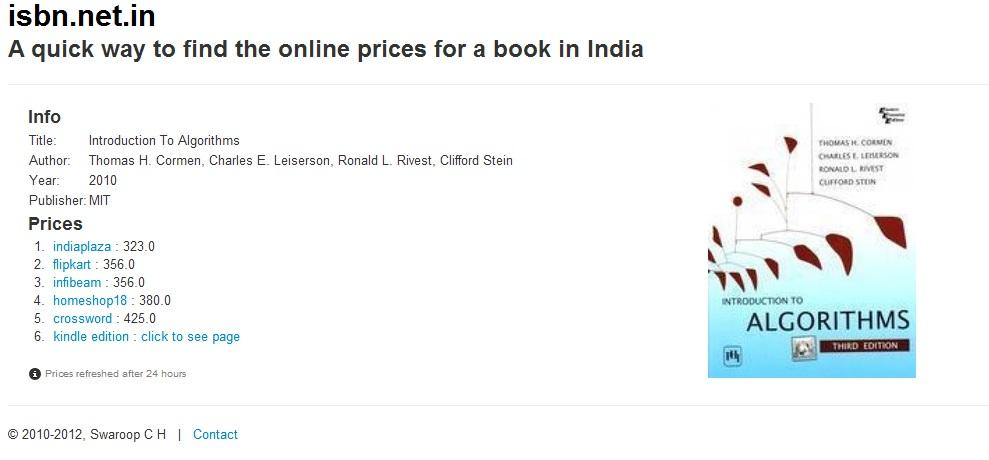
\includegraphics[width=16cm]{fig/book_price.jpg}
  \caption[Example of price comparasison mashup]
  { a mashup for finding online price for a book from various shopping sites. The results of a query of an ISBN number are displayed above.}
\end{figure}
\clearpage

Some mashups are categorized in terms of data visualization for instance where the data is simply displayed in an appealing way using various visualization techniques. Facebook’s timeline feature can  serve as an example of a data visualization mashup since it just takes the data and presents it in a timestamp based format akin to the data entries in chronological order. There are some image search engines which can display items visually in lists, graphs etc. and use some item-related attributes such as dates of last uploaded, prices, items of rank based order \cite{1}.

We focus mainly on data aggregating mashups since we are striving to design our semantic mashup by extracting data from multiple sources and finding ways to collate it by adding semantics. More emphasis is placed on the extraction strategies and we shall look into them in the later part of this chapter.

\section{Approaches to mashup development}
Here, we discuss the various tools and programming methodologies used in creating the mashups that we see today. They mostly involve widget tools, web technologies etc.

\subsection{Widget based tools}
There are a variety of software tools online that boast ease of use, helpful for non-programmers and rapid development of dynamically enhanced mashups. The research paper Mash maker: Mashups for the masses described it as an interactive tool which can be used to edit, manipulate, query and visualize live semi-structured data \cite{13}. The main advantage of using mashup making tools is that no prior experience of programming is needed as non-experts can use it effectively. However, the problems associated with using these kind of tools is that the user will have many restrictions and in some cases, the data will have to be live and visualizations and manipulations can be done only to some extent.

Some of the famous tools like Yahoo pipes, Microsoft Popfly and Dapper from \cite{14} claim that users with no programming background can easily use these tools to develop mashups on their own. Microsoft Popfly is deprecated as of now. Yahoo pipes relies heavily on RSS feeds and uses a widget approach where users can choose existing widgets that perform specific operations and they can be customized \cite{14}. Some of the problems associated in using these are that it will be difficult to keep track of all the widgets involved and since the widgets are pre designed for specific purposes, they may not support any new purposes. Even though mashups are designed using these tools, the created mashups are restricted to only some kind of functionality that can be made with respect to the preformatted widgets used in these tools.

There exist some tools that can be used for specific purposes such as data extraction. Mashup enablers help in extracting content from different web sites without any need for novice knowledge. These tools can be used effectively for web sites whose layouts get changed constantly and the main advantage is that they provide access to the unstructured content of web pages which would otherwise have been difficult to achieve as specified in \cite{15}.

However, these tools will not be effective, as they can only extract parts of website that are easily recognizable via the web pages source code. They will benefit in gathering information for mashups but the thesis project involves case studies of extracting data from unstructured web pages, the queries involved are being user generated, and thus the outcomes can get changed based on different user queries.

\subsection{ Web technologies}
Some of the research papers explained about the most important web technologies that can be used in developing mashups. A widely used tool is Asynchronous JavaScript over XML (AJAX) which is appropriate for developing mashup applications due to its real time syndication. There are several advantages using specific tools in \cite{16}, for instance they can also be useful for data to be integrated across web feeds, various sites etc. To satisfy the thesis objectives, a Python web framework was used to support dynamic display, and processing of asynchronous data retrieval XML http requests.

JavaScript is very useful for designing mashups since most of the APIs are coded in JavaScript. For instance, Google search API is written in JavaScript. It’s also the scripting language of the web and is useful for adding dynamic functionalities in web pages.

For selecting a suitable web programming language, we chose Python for its simplicity and ease of use. It is soon becoming the \textsl{de facto} programming language for the web. With respect to our goals in the project regarding data extraction, \cite{5} and \cite{6} are popular Python libraries, which make it easier to extract data from HTML and XML files. The documentation has several examples which were researched akin to our project goals and were well correlated. Programming the focused scraper also gives us more control over our mashup design and hence,-  a versatile application can be built catering to the needs of the user specific queries.

\subsection{APIs and web services}
As already said, the most widely used API in mashups is Google maps. This can be found in a wide variety of mashups where it requires the location to be displayed. Amazon has also made its API freely and publicly accessible and, as said, can be used to display their content \cite{17}. The Google search API is another famous interface which can be implemented, such that Google search results can be displayed in the mashup and it can be programmed to provide specific results based on keyword searches.

Although the API’s have user friendly tutorials with lot of examples catering to the needs of any kind of user, its required that the user should be skilled at least in an intermediate level of a programming language, in order to use these APIs effectively. Therefore, a relatively detailed knowledge of a  programming language is required, in order to integrate these API’s into ones mashup application.

Not all of the websites will have an API, and often other techniques are required to extract the data one needs. There are also ethical and social challenges involved, if websites don’t want to share their data with other parties \cite{4}.

\subsection{Screen scraping}
Due to lack of APIs for some webpages, screen scraping is a useful technique in retrieving the information from the data sources. As the name implies, it is the process of parsing and analyzing the source code of a web page, in order to extract the semantic structure of the data. In our project context, web scraping is more appropriate, since we deal with HTML web pages, and thus it represents a useful technique in accordance to our project goals.

Despite the merits, \cite{4} specifies that there are some issues with this method. For instance, the scraping method should be modeled akin to the source code of the web page, and this could prove difficult, if different web pages are created by using different formats. Web sites often undergo changes in representing their data in order to get a different visual feel and this can hinder the scraping tool’s chances of successful extraction of data. In our project, we aim to deal with a challenge such as this and we illustrate case studies for a website with one format and a second website with a different format.


\section{Problems with mashups}
Some of the research papers referred to how mashups benefit users as well as what kind of problems did the mashup developers encounter. Most of the problems that occur were due to the reliability of the API to be used, its documentation and issues with coding the mashup \cite{8}. Even though an API exists for a web site that is to be mashed up, this doesn't guarantee ease of use of wide take-up, as there might be some problems with understanding the documentation of the API \cite{19}.

\cite{4} indicated some data integration challenges. This mainly refers to issues which can be encountered with the data involved. There might be issues with the data models and sometimes with the data itself. Due to the source models being third party, mashup developers may not be familiar with them. Some of the data may either be missing or not suitable for automation into the mashup and hence, additional preprocessing is required. This is where semantic modeling comes in as stipulated in \cite{4}.

Moreover, there are several open challenges regarding the usage of data, from social and, ethical points of view. Any data used will have to be referred back to the original source. Some content providers will have control of its data as intellectual property and will instigate a fair use policy \cite{4}. These shouldn’t be much pondered upon as long as content owners’ guidelines are met.


\section{Web scrapers vs web crawlers}

Web scraping is plausibly different from web crawling. The former denotes information retrieval from websites with emphasis on data. Web scraping mainly deals with transforming unstructured data from html pages to readable data. Web crawling usually deals with indexing the web with web pages related to some domain. Research on web scraping came to light in \cite{22}, which aimed to combine data and services from web sources with a dedicated tool. This tool can be useful in accomplishing the data extraction tasks, after which data are present individually as web output. Its emphasis is placed on data. It provides operators to take relevant data as input, process it via a data flow architecture that can add metadata. The output is provided on a spreadsheet, which is later processed by end user to add to required services (like maps, for instance) and is published as output.
